\documentclass{article}
\usepackage[utf8]{inputenc}
\usepackage{amsmath}
\usepackage{listings}
\usepackage{graphicx}

\title{Bloom Filter}
\author{ Yannick Koller & Mike Gilgen }
\date{November 2022}

\begin{document}
\maketitle

\section{Einleitung}
Der Bloom Filter, benannt nach dem Erfinder Burton Howard Bloom, ist eine Datenstruktur die auf die Wahrscheinlichkeit basiert. Dies macht diese Datenstruktur sehr Speichereffizient, da die unnötigen Diskzugriffe um einen Bruchteil reduziert. Ein Nachteil, gegenüber den bekannten Datenstrukturen, ist jedoch die Fehleranfällig dieser Datenstruktur. Trotzdem findet sie in der Praxis viele Anwendung, weil sie so effizient ist und in gewissen Bereichen es gar nicht nötig ist 1:1 die Daten abzufragen.

\section{Vor- und Nachteile}
Hier ein paar Vor- und Nachteile
\begin{center}
\begin{tabular}{c|c}
    Vorteil & Nachteil \\
    \hline
    Speichereffizient & Fehleranfällig \\
\end{tabular}
\end{center}
Die Fehleranfälligkeit gilt allerdings nur für Abgefragte Elemente die sich nicht in der Menge im Speicher befindet. Zu diesem Fehler kommt es, wenn ein abgefrages Element ein "Hash-Overlap", also den gleichen Hashwert hat, wie ein Wert in der Menge. Für alle gesuchten Elemente, die sich nicht in der Menge befinden, kann man dafür eine klare Aussage machen, dass sie nicht in der Menge ist. Daraus folgen zwei Aussagen die diese Datenstruktur zurückgibt wenn man ein Element abfrägt:

\begin{itemize}
    \item Is probably in set (positive)
    \item Is definitely not in set (negative)
\end{itemize}

\clearpage

\section{Praxisbeispiel}
Der Google Webbrowser Chrome benützt den Bloomfilter um URLs durch die potenziell Malware verbreitet wird zu untersuchen. Malwarescans sind sehr rechenaufwändig, vor allem wenn diese Malware noch nicht bekannt ist. Darum wird beim Chrome jede URL erst durch den Bloomfilter überprüft und nur wenn es ein positives Resultat erzeugt, wird die URL komplett untersucht.

\section{Funktionsweise}
Die Funktionsweise des Bloomfilters ist am besten durch den verwendeten Algorithmus zu erklären. Folgende Komponenten sind dabei notwendig:

\begin{itemize}
    \item Bit-Array mit $m$ Bits
        \begin{itemize}
            \item{Dieser dient als Filter}
        \end{itemize}
    \item Gewünschte Fehlerquote $p$
    \item Anzahl Hashfunktionen $k$
    \item Array für alle verwendeten Hashfunktionen
\end{itemize}

Die aufgelisteten Variablen können mit folgenden Formeln berechnet werden:

\begin{equation}
    m = -\frac{n \ln{p}}{(\ln{2})^2}
\end{equation}
\begin{equation}
    k = \frac{m}{n} \ln{2}
\end{equation}
\begin{center}
    \textit{Die Herleitung de Formeln sind in Wikipedia zu finden.}
\end{center}
Sind diese Variabeln bekann kann der Filter aufgebaut werden.
\begin{center}
    \textit{pseudo Code}
\end{center}
\begin{lstlisting}
    // defining the Arrays
    HashFunctions[] hashFunctions;
    boolean[] filter;

    // defining the Hashalgorithms and build an empty filter
    boolean[] buildFilter(int n, double p){
        int m = (int) -((n * Math.log(p)) / (Math.log(2) * Math.log(2)));
        int k = (int) ((m / n) * Math.log(2));

        hashFunctions = new HashFunction[k];
        // feeding the filter
        for( int i = 0; i < k; i++ ) {
            hashFunctions[i] = Hashing.<hashAlogrithm>(RandomInt);
        }
        filter = new boolean[m] // empty filter
    }
\end{lstlisting}
Nun steht der Filter und die Hashing Algorithmen für die Datenstruktur sind definiert. Jetzt muss der Filter nur noch die richtigen Bits gesetzt haben. Dafür dient folgende Methode:
\begin{lstlisting}
    void add(E element){
        for( HashFunction hashFunction : hashFunctions ){
            filter[hashFunction(element)] = true;
        }
    }
\end{lstlisting}
Für jedes Element das hinzugefügt wird, wird an jedem Index der durch die Hash Funktionen zurückgegeben wird der Wert auf $true$ gesetzt. \\
Bei der Abfrage ob nun ein gesuchtes Element in der Datenstruktur enthalten ist, kann nun der Filter auf dieselbe Weise abgefragt werden.

\begin{lstlisting}
    boolean mightContain(E element){
        for( HashFunction hashFunction : hashFunctions ){
            if( !filter[hashFunction(element)] ){
                return false;
            }
        }
        return true;
    }
\end{lstlisting}
Wenn nur eine Stelle im Filter $false$ ist weiss man, dass sich das Element garantiert nicht in der Menge befindet. Andernfalls gilt die Wahrscheinlichkeit $p$, dass sich das Element in der Menge befindet.

\clearpage

\section{Erkenntnisse aus unserem Projekt}
Wir testeten unser Filter mit der eigenen Liste indem wir jeweils nur jeden ungeraden Index in den Filter aufnahmen, mit einer False-Positive Wahrscheinlichkeit $p = 0,2$. Die False Positives zählten wir, indem wir nun jeden geraden Index abfragten, also jede Abfrage war ein Mismatch. Dadurch variierte die Anzahl der False Positives zwischen 5600 und 5900 und die False Positives Rate schwankte um $0,2 \pm 0,01$ herum. Die False Positives Rate entspricht somit ziemlich genau der definierten Wahrscheinlichkeit $p = 0,2$. Die Anzahl der False Positives ist in demfall auch gleich die Anzahl der Hashing-Overlaps.
\begin{figure}[h!]
    \centering
    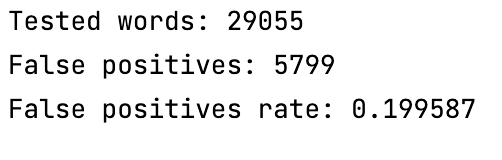
\includegraphics{./lib/dist_bloomResult.png}
    \caption{Bloom Result}
    \label{fig:Bloom Result}
\end{figure}

\end{document}
